%%%%%%%%%%%%%%%%%%%%%%%%%%%%%%%%%%%%%%%%%%%%%%%%%%%%%%%%%%%%%%%%%%%%%%%%%%%%%%%
% Chapter 4 : Título del Capítulo cuatro
%%%%%%%%%%%%%%%%%%%%%%%%%%%%%%%%%%%%%%%%%%%%%%%%%%%%%%%%%%%%%%%%%%%%%%%%%%%%%%%
\section{Descripción de las Funciones Propuestas por el GenOpt}
\label{sec:GENOPT}

El concurso \textit{GenOpt} ha propuesto un total de \textbf{18 funciones} de dimensiones $D = 10, 30$ a optimizar. A partir de sus características, estas funciones se pueden agrupar en tres familias diferentes: 

\bigskip
\subsection{Funciones GKLS}\label{sec:GKLS}
Las funciones GKLS \cite{GKLS} son obtenidas mediante un generador de funciones de tres tipos (no-diferenciable, continuamente diferenciable y dos veces continuamente diferenciable) con mínimos locales y globales conocidos.
 
\subsection{Funciones clásicas transformadas}

Esta familia de funciones se obtienen realizando una transformación a aquellas funciones clásicas para probar métodos de optimización global continua como son:
    \begin{itemize}
    	\item Rastrigin, $D = 10, 30$ \\
    		\begin{equation}\label{eq:rastrigin}
					f(x) = An + \sum^{d}_{i=1}{[x^{2}_{i} - A \cos{2\pi x_{i}}]}
 					\end{equation}
    	\item Rosenbrock, $D = 10, 30$ \\
    	    \begin{equation}\label{eq:rosenbrock}
					f(x,y) = (a - x)^{2} + b(y - x^{2})^{2}
 					\end{equation}
    	\item Zakharov, $D = 10, 30$ \\
    	    \begin{equation}\label{eq:zakharov}
					f(x) = \sum^{d}_{i=1}{x_{i}^{2}} + (\sum^{d}_{i=1}{0.5ix_{i}})^{2} + (\sum^{d}_{i=1}{0.5ix_{i}})^{4}
 					\end{equation}
    \end{itemize}
    Cada función \textit{x} es transformada en cada instancia de la siguiente manera: 
    \begin{equation}
    x' = Mx + x_{0}
    \end{equation}
    Dónde $x_{0}\in[-0.1, 0.1]^{D}$ es un translación aleatoria y M es una matriz ortogonal con número de condición igual a 100.

\subsection{Funciones compuestas} 

Por último, en esta familia encontraremos funciones obtenidas a partir de la composición de las funciones de la segunda familia. Estas funciones se construyen seleccionando aleatoriamente \textit{n} funciones clásicas $f_{1},...,f_{n}$ del siguiente conjunto: 
    	  \begin{itemize}
    	  	\item Goldstein-Price, $D_{f} = 2$;
    	  	\item Hartmann, $D_{f} = 3; 6;$
    	  	\item Rosenbrock, $D_{f} = rand(3, D/2);$
    	  	\item Rastrigin, $D_{f} = rand(3, D/2);$
    	  	\item Sphere, $D_{f} = rand(3, D/2);$
    	  	\item Zakharov, $D_{f} = rand(3, D/2);$
    	  \end{itemize}
    La suma de las dimension $D_{f_{1}},...,D_{f_{n}}$ debe cumplir que $\sum_{i}{D_{f_{i}}} = D$. \\
    Una función \textit{x} es sujeta a un roto-translación tal que, para cada instancia: 
    \begin{equation}
    	x' = Ux + X_{0}
    \end{equation}
    Dónde $U$ es una matriz ortogonal aleatoria y $x_{0}\in[-0.1, 0.1]^{D}$ es una pequeña translación aleatoria. El valor de cada instancia es calculado como: 
    \begin{equation}
    	f(x) = c + \sum^{n}_{i=1}{f_{i}(x'_{b_{i}},...,x'_{b_{i}} + D_{f_{i}} - 1)}
    \end{equation}
    Dónde $b_{i} = \sum^{i-1}_{j=1}{D_{f_{i}}}$. \\
    En la siguiente figura podemos observar un esquema de este proceso: 
    	  \begin{figure}[!ht]
  				\centering
					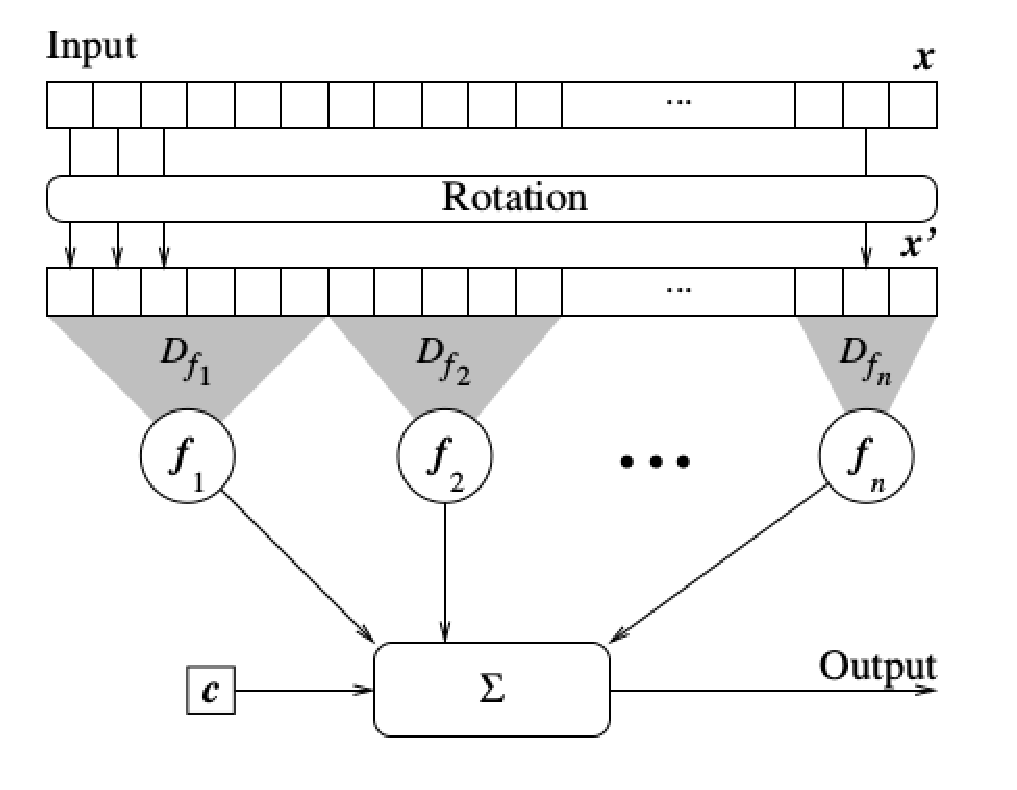
\includegraphics[scale=0.5]{images/composicion}
  				\caption{Composición de funciones.}
				\end{figure}

\newpage

%%%%%%%%%%%%%%%%%%%%%%%%%%%%%%%%%%%%%%%%%%%%%%%%%%%%%%%%%%%%%%%%%%%%%%%%%%%%%%
\section{Estudio de la Parametrización}
\label{sec:PARAM}
%%%%%%%%%%%%%%%%%%%%%%%%%%%%%%%%%%%%%%%%%%%%%%%%%%%%%%%%%%%%%%%%%%%%%%%%%%%%%%
\section{Análisis de Rendimiento}
\label{sec:PERFORMANCE}
